%!TEX root = ../../main.tex

\chapter{Das erste Kapitel}
Dies ist der Text des ersten Kapitels.
Nur erwähnte Literaturverweise werden auch im Literaturverzeichnis abgebildet: \cite[S.12 ff]{baumgartner:2002}, \cite[S.1-3]{dreyfus:1980}

Fußnote\footnote{Mit Fußnoten können Begriffe erklärt werden, die dem Leser bereits bekannt sein könnten}.

\begin{wrapfigure}{r}{.4\textwidth}
    \centering
    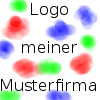
\includegraphics[height=.1\textwidth]{logo.png}
    \vspace{-10pt}
    \caption{Das Logo der Musterfirma\footnotemark}
\end{wrapfigure}
\footnotetext{aus \cite{mustermann:2012}}
Lorem ipsum dolor sit amet, consetetur sadipscing elitr, sed diam nonumy eirmod tempor invidunt ut labore et dolore magna aliquyam erat, sed diam voluptua.
At vero eos et accusam et justo duo dolores et ea rebum.
Stet clita kasd gubergren, no sea takimata sanctus est Lorem ipsum dolor sit amet.
Lorem ipsum dolor sit amet, consetetur sadipscing elitr, sed diam nonumy eirmod tempor invidunt ut labore et dolore magna aliquyam erat, sed diam voluptua.
At vero eos et accusam et justo duo dolores et ea rebum.
Stet clita kasd gubergren, no sea takimata sanctus est Lorem ipsum dolor sit amet.

Mit LaTeX können Formeln gut dargestellt werden, siehe \ref{eq:example1}
\begin{equation}
    t-t_{0}=\sqrt{\frac{l}{g}}\int_{0}^{\varphi}{\frac{d\psi}{\sqrt{1-k^{2}\sin^{2} {\psi}}}} = \sqrt{\frac{l}{g}} F(k,\varphi)
    \label{eq:example1}
\end{equation}

LaTeX bietet die Möglichkeit von geordneten und ungeordneten Listen.
\begin{enumerate}
    \item Erster Punkt.
    \item Zweiter Punkt.
    \item {Dritter Punkt.}
\end{enumerate}
\begin{itemize}
    \item Erster Punkt.
    \item Zweiter Punkt.
\end{itemize}

Jede weitere wird nur verlinkt: \acf{AGPL}~\cite{fsf:2007}
Verweise auf das Glossar: \gls{Glossareintrag}, \glspl{Glossareintrag}

